\chapter{Wprowadzenie}
\label{cha:wprowadzenie}

%---------------------------------------------------------------------------
\section{Cel pracy}
\label{sec:celePracy}


%---------------------------------------------------------------------------
\section{Obecnie dostępne narzędzia}
\label{sec:dostepneNarzedzia}

%===========================================================================
\chapter{Szczegóły implementacyjne}
\label{sec:zastosowanePodejscie}
Jednym z celów projektu jest umożliwienie wykonania parsowania i wygenerowania dokumentacji bez konieczności
instalacji zewnętrznych narzędzi (jakim byłby na przykład \textit{protoc}). Aby sprostać temu wymaganiu konieczna jest implementacja parsera 
języka Protocol Buffers jako części JVM, nie wołając poza nią. Podjęto decyzję wykorzystania \textit{Scala Parser Combinators} (,,kombinatorów parserów'').


%---------------------------------------------------------------------------
\section{Parser}
\subsection{Wprowadzenie do kombinatorów parserów}
TODO klasyfikacja, opisać że są lewo stronnie rekurencyjne etc.

\verb|http://en.wikipedia.org/wiki/Recursive_descent_parser|

\verb|http://en.wikipedia.org/wiki/Left_recursion|
\verb|http://en.wikipedia.org/wiki/Parser_combinator|

\verb|http://stackoverflow.com/questions/17840/how-can-i-learn-about-parser-combinators|

\subsection{Fragmenty implementacji}
Przedstawić fragmenty parsera. Najlepiej go dać jako dodatek jednak w całości.

Parser w tym projekcie budowany jest za pomocą części języka \textit{Scala} zwaną \textit{,,Parser Combinators''}.

\begin{lstlisting}
def messageTypeDef: Parser[ProtoMessageType] = opt(comment) 
                                               ~ "message" ~ ID ~ "{" 
                                               ~ rep(enumTypeDef | instanceField | messageTypeDef) 
                                               ~ "}" ^^ {
  case maybeDoc ~ m ~ id ~ p1 ~ allFields ~ p2 =>
    // utworzenie instancji ProtoMessageType
}
\end{lstlisting}


%---------------------------------------------------------------------------
\section{Verifier}
Generalny opis dlaczego musiał powstac

Przedstawić jakie sprawdzania obsługuję. 
Pokazać że obsługuję importy oraz udowodnić dlaczego konieczny jest dodatkowy krok na to.
No bo bez takiego kroku nie wiedziałbym czy przypadkiem gdzies indziej nie zostal zdefiniowany jakis message etc.

\subsection{Obsługiwane weryfikacje}
Moze sub sectiony o tych checkach oraz konkretne przykłady błędów i jak są komunikowane?


%---------------------------------------------------------------------------
\section{CodeGenerator}
Generator kodu w tym przypadku jest bardzo prostą serią transformacji.
Opisać, wspomnieć że korzystam z mustache etc.

\subsection{Zrzuty ekranu wygenerowanej dokumentacji}
\label{sec:screenshots}

\begin{center}
 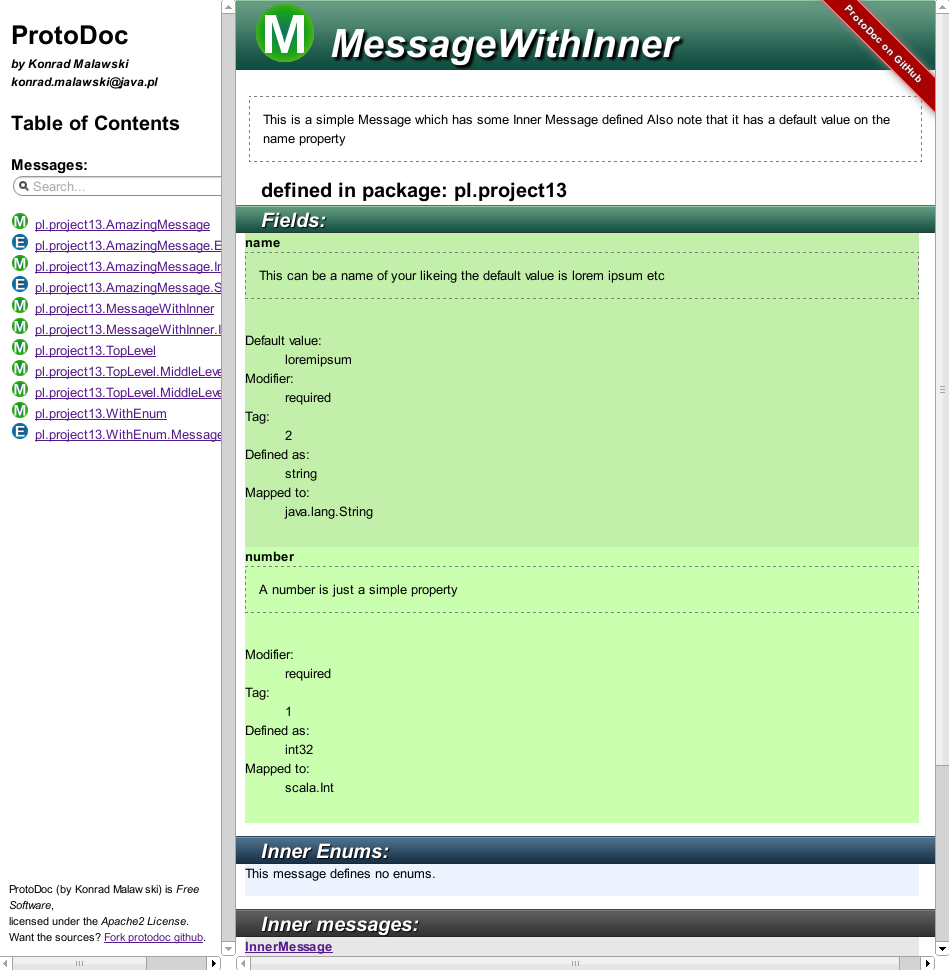
\includegraphics[width=\textwidth]{../protodoc_main.png}
 % protodoc_main.png: 949x970 pixel, 93dpi, 25.92x26.50 cm, bb=0 0 735 751
\end{center}

%===========================================================================
\chapter{Zastosowanie ProtoDoc do automatyzacji dokumentacji projektów}

%===========================================================================
\chapter{Przykład}
Podajemy takie wejście:
\begin{verbatim}
message Person {
  required int32 id = 1;
  required string name = 2;
  optional string email = 3;
}
\end{verbatim}

Następnie wykonanie:

A ostatecznie otrzymujemy taką stronę: \verb|http://protodoc.project13.pl/sample|.

%TODO Tutaj screeny gotowego 
